% A sample model to write a TFG project

% IMPORTANT!!! Substitute "draft" with "final" to render the final version of the TFG 
\documentclass[titlepage,openright,twoside,a4paper,draft,12pt,french]{book}

% Configuring the environment to support spanish characters.
\usepackage[utf8]{inputenc}
\usepackage[T1]{fontenc}
\usepackage[frenchb]{babel}
\selectlanguage{french}

\usepackage[pdftex,final]{graphicx}

% Style package
\usepackage{trinidad-TfG}
% Font Package (Palatino)
\usepackage{mathpazo}
% Packages for specific capabilities
\usepackage{rotating} % for text rotation in tables
\usepackage{multirow} % for multirow in tables
\usepackage{subfigure} % Place subfigures in figure environment
% Packages for specific symbols
\usepackage{amssymb}
\usepackage{amsmath}
\usepackage{amsfonts}
\usepackage{eurosym} % Euro symbol
\usepackage{bbding} % for \XSolidBrush
\usepackage{pifont} % for \ding{55} (a check mark)

%Defining the folders on the images
\graphicspath{ {figures/Chap2/} }

\author{Nombre del Alumno}{Grado en Ingeniería Informática - Especialidad}{D.~}{12345678A}
\authorURL{http://www.lsi.us.es/~trinidad}
\authorEMail{fmenekeu@gmail.com}
\setTitle{Rapport de Stage Pré-ingénieur}
%\setSubtitle{No subtitle}
\setUniversity{Ecole Polytechnique de Yaoundé}
\copyrightText{Pon aquí cuestiones acerca del copyright}
\supervisor{MAHI NKAK Paul}{Ing.~}{Manager Département Consulting}



\makeglossaries
\begin{document}
\makeTitlePage

\pagestyle{empty}
\begin{dedication}
Tu dedicatoria aquí
\end{dedication}
\pagenumbering{roman}
\pagestyle{trinidadPhD}

\chapter*{Agradecimientos}

Section des Remerciements 
\chapter*{Resumen}
Un resumen de un párrafo sobre el problema planteado en el proyecto y la solución. Máximo 300 palabras.

\tableofcontents
\listoffigures
\listoftables
\listoftodos
\newpage

\pagenumbering{arabic}
\newacronym{pl}{PL}{Product Line}
\newacronym{spl}{SPL}{Software Product Line}
\newacronym{aafm}{AAFM}{Automated Analysis of Feature Models}
\newacronym{aasfm}{AASFM}{Automated Analysis of Stateful Feature Models}
\newacronym{fm}{FM}{Feature Model}
\newacronym{efm}{EFM}{Extended Feature Model}
\newacronym{cbfm}{CBFM}{Cardinality-Based Feature Model}
\newacronym{dspl}{DSPL}{Dynamic Software Product Line}
\newacronym{AI}{AI}{Artificial Intelligence}
\newacronym{csp}{CSP}{Constraint Satisfaction Problem}
\newacronym{cop}{COP}{Constraint Optimisation Problem}
\newacronym{sla}{SLA}{Service-Level Agreement}
\newacronym{mas}{MAS}{Multi-Agent System}
\newacronym{eo}{EO}{Explanatory Operation}
\newacronym{fol}{FOL}{First Order Logic}
\newacronym{kb}{KB}{Knowledge Base}
\newacronym{cwa}{CWA}{Closed World Assumption}
\newacronym{atl}{ATL}{Atlas Transformation Language}
\newacronym{mde}{MDE}{Model-driven Engineering}
\newacronym{sfmm}{SFMM}{Stateful Feature Metamodel}
\newacronym{sfm}{SFM}{Stateful Feature Model}
\newacronym{steam}{STEAm}{STateful fEature model Analyser}

\newcommand{\fm}{\Gls{fm}\xspace}
\newcommand{\fms}{\Glspl{fm}\xspace}
\newcommand{\efm}{\Gls{efm}\xspace}
\newcommand{\efms}{\Glspl{efm}\xspace}
\newcommand{\cbfm}{\Gls{cbfm}\xspace}
\newcommand{\cbfms}{\Glspl{cbfm}\xspace}
\newcommand{\spl}{\Gls{spl}\xspace}
\newcommand{\spls}{\Glspl{spl}\xspace}
\newcommand{\aafm}{\Gls{aafm}\xspace}
\newcommand{\aasfm}{\Gls{aasfm}\xspace}
\newcommand{\dspl}{\Gls{dspl}\xspace}
\newcommand{\dspls}{\Glspl{dspl}\xspace}
\newcommand{\eo}{\Gls{eo}\xspace}
\newcommand{\fol}{\Gls{fol}\xspace}
\newcommand{\kb}{\Gls{kb}\xspace}
\newcommand{\cwa}{\Gls{cwa}\xspace}
\newcommand{\cop}{\Gls{cop}\xspace}
\newcommand{\cops}{\Glspl{cop}\xspace}
\newcommand{\csps}{\Glspl{csp}\xspace}
\newcommand{\csp}{\Gls{csp}\xspace}
\newcommand{\toolname}{\Gls{steam}\xspace}
\newcommand{\atl}{\Gls{atl}\xspace}
\newcommand{\mde}{\Gls{mde}\xspace}
\newcommand{\sfmm}{\Gls{sfmm}\xspace}
\newcommand{\sfm}{\Gls{sfm}\xspace}
\newcommand{\sfms}{\Glspl{sfm}\xspace}

\part{Introdution}
%!TEX root =  tfg.tex
\chapter{Introduction}

\begin{quotation}[Novelist]{Ernest Hemingway (1899--1961)}
The good parts of a book may be only something a writer is lucky enough to overhear or it may be the wreck of his whole damn life -- and one is as good as the other.
\end{quotation}

\begin{abstract}
Resumen de lo que va a ocurrir en el capítulo. ¿Cuál es el objetivo que tenemos con este capítulo?
\end{abstract}

\section{Contexte}

Le 14 Avril 2016, une nouvelle règlementation sur la protection des données à caractère personnel est entrée en vigueur ; laissant une marge de deux années à toute entreprise manipulant des données à caractère personnel d’individus ressortissant de l’UE le soin de s’y conformer. Mazars Cameroun, branche de Mazars Group, a décidé de se conformer à cette réglementation entrée en vigueur le 25 Mai 2018. Cette mise en conformité a pour principal objectif d’accroître à la fois la sécurité des données à caractère personnel manipulées par l’entreprise mais aussi, de responsabiliser les acteurs de ce traitement. Ainsi donc, la classification des informations manipulées est incontournable pour la mise en conformité de l’entreprise. 

\section{Problématique}

Classifier une donnée c’est lui attribuer une mention qui permet de caractériser la valeur et l’importance stratégique de cette donnée détenue par une entreprise et, conséquemment le niveau de protection à lui accorder.

Comment mettre en place une solution de classification efficace qui va pouvoir garantir la sécurité des informations manipulées au sein de Mazars Cameroun ? 

Quelles sont les différentes procédures à mettre sur pied afin d’assurer la mise en conformité de Mazars Cameroun non seulement au RGPD, mais aussi aux lois en vigueur ?


\section{Objectifs et Motivations}

Les objectifs visés par la classification des données manipulées au sein de Mazars Cameroun sont les suivants :
\begin{itemize}
  \item Accroître la protection des données à caractère personnel manipulées au sein de la structure ;
  \item Responsabiliser les acteurs du traitement de ces données ;
  \item Renforcer les droits des personnes ;
  \item Crédibiliser la régulation.
\end{itemize}

Comme motivations à ce projet de mise en conformité, la première est les sanctions prévues par le RGPD en cas de non-conformité ; ces sanctions peuvent aller jusqu’à une amende de 20 Millions d’Euros. En plus, la mise en conformité au RGPD est un critère non négligeable requis par certains clients en ce qui concerne l’acquisition de nouveaux marchés. Par ailleurs, la mise en conformité RGPD est un service que pourrait proposer la structure mais il faudrait premièrement qu’elle-même y soit conforme. 

\part{Concepts théoriques et méthodologiques}
%!TEX root =  tfg.tex
\chapter{Concepts théoriques et méthodologiques}

\begin{quotation}[Novelist]{Ernest Hemingway (1899--1961)}
The good parts of a book may be only something a writer is lucky enough to overhear or it may be the wreck of his whole damn life -- and one is as good as the other.
\end{quotation}

\begin{abstract}
Resumen de lo que va a ocurrir en el capítulo. ¿Cuál es el objetivo que tenemos con este capítulo?
\end{abstract}

\section{Présentation du RGPD}
\subsection{Origines}
Le Règlement Général sur la Protection des données en abrégé RGPD est une loi qui concerne la protection des données personnelles des utilisateurs habitants d’un pays de l’Union Européenne. Il vient remplacer la Directive sur la protection des données personnelles adoptée en 1995. Le RGPD a été finalement adopté par le Parlement Européen le 14 Avril 2016 ; ses dispositions sont applicables dans tous les états membres de l’Union Européenne à compter du 25 Mai 2018.

Il est important de noter que le RGPD s’applique [1]:
\begin{itemize}
   \item[•] Aux entreprises ou entités qui traitent des données à caractère personnel dans le cadre des activités de l’une de leurs filiales établie au sein de l’UE, indépendamment de l’endroit où sont traitées les données ;
   \item[•] Aux entreprises établies en dehors de l’UE qui proposent des biens ou services (payants ou gratuits), ou surveillent le comportement des personnes dans l’UE.
\end{itemize}

\subsection{Objectifs}
Le RGPD a les différents objectifs suivants [2] :
\begin{itemize}
   \item[•] Renforcer le droit des personnes;
   \item[•] Responsabiliser les acteurs traitants les données;
   \item[•] Crédibiliser la régulation.
\end{itemize}
L’on peut donc retenir que les principaux objectifs du RGPD sont d’accroître à la fois la protection des personnes dont les données à caractère personnel sont traitées et de responsabiliser les acteurs de ce traitement. 
\subsection{Principes}
Le type et la quantité de données à caractère personnel qu’une entreprise/organisation peut traiter dépendent de la raison pour laquelle elles sont traitées et le but dans lequel elles le sont. Ainsi, l’entreprise/organisation doit respecter un certain nombre de principes [3] :
\begin{itemize}
   \item[•] Les données personnelles doivent être traitées de manière licite et transparente : \textbf{licéité, loyauté et transparence};
   \item[•] Il doit y avoir des finalités précises pour traiter des données et l’entreprise/organisation doit indiquer ces finalités aux personnes dont les données sont collectées : \textbf{limitation des finalités};
   \item[•] \textbf{Minimisation des données:} l’entreprise ne peut traiter que les données personnelles qui sont nécessaires pour atteindre ces finalités ;
   \item[•] \textbf{Exactitude:} L’entreprise doit s’assurer que les données personnelles collectées sont exactes et mises à jour ;
   \item[•] L’entreprise ne peut utiliser les données collectées pour d’autres finalités qui ne sont pas compatibles avec celles pour lesquelles elles ont été initialement collectées ;
   \item[•] \textbf{Limitation de la conservation:} les données collectées ne doivent pas être gardées plus longtemps que nécessaires ;
   \item[•] \textbf{Responsabilité:} l’on doit pouvoir démontrer la conformité de l’entreprise avec le RGPD, mener une analyse d’impact relative à la protection des données, …
   \item[•] \textbf{Limitation des transferts:} pas de transfert de données d’un territoire à l’autre à moins que ce pays ou territoire assure un niveau de protection adéquat des droits et libertés des propriétaires des données ;
   \item[•] \textbf{Intégrité et confidentialité:} l’entreprise doit mettre en place des mesures techniques et organisationnelles afin de garantir la sécurité des données collectées.
\end{itemize}
\subsection{Sanctions en cas de non-conformité}
En cas de non-respect du RGPD, l’entreprise/organisation s’expose aux sanctions suivantes :
\begin{itemize}
  \item[•] \textbf{20 millions d'Euros} pour les PME;
  \item[•] Jusqu’à plusieurs milliards d’euros pour les grands groupes, il s’agit plus précisément de \textbf{4\% du chiffre d'affaires} global du groupe.
\end{itemize}

\section{Méthodologie}

L’information est d’une importance capitale dans une entreprise. Pouvoir tracer le cycle de vie de l’information est une activité incontournable afin de protéger et sécuriser celle-ci.

Afin d’aboutir à une solution de classification des données de l’entreprise, nous avons suivi un ensemble d’étapes [4].

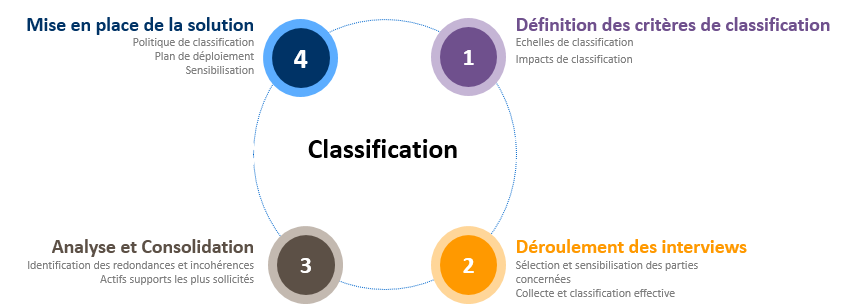
\includegraphics{methodologie.png}

\begin{enumerate}
   \item \textbf{Définition des critères de classification des données}
   \begin{enumerate}
     \item \textbf{Echelles de classification}
     
     Le but de la classification des données est de garantir la sécurité des données sans entraver la fluidité de l’information et des processus de l’entreprise. Pour se faire, il est important de définir des échelles de classification se basant sur les 3 concepts de la sécurité : la confidentialité, l’intégrité et la disponibilité.
     \item \textbf{Impacts de classification}
     
     En entreprise, les informations sont identifiées suivants des niveaux d’exposition au risque et de granularité (groupes d’information, données élémentaires, …). Ainsi l’impact associé en cas de divulgation ou d’altération sera fonction de ces niveaux. Les impacts de la perte de confidentialité, d’intégrité et de disponibilité de l’information sont intriqués.  Ces impacts peuvent présenter pour l’entreprise des défis pour sa conformité légale, réglementaire et contractuelle, ses opérations quotidiennes, sa réputation ou ses finances. Nous avons donc choisi de catégoriser les impacts ainsi que  montre la figure suivante : Voir annexe 1.
   \end{enumerate}
   \item \textbf{Déroulement des interviews}
   \begin{enumerate}
       \item \textbf{Sélection et Sensibilisation des partis concernés}
       
       Pour mener à bien cette activité de classification, il est important de choisir les interlocuteurs compétents et qualifiés, ayant autorité de décision sur les processus et informations pour lesquels ils sont sollicités. Une étape de sensibilisation afin de préparer l’interlocuteur à fournir les informations pertinentes pour une bonne classification.
       \item \textbf{Collecte et classification des informations}
       
       Les informations ont été collectées à travers des interviews des interlocuteurs choisis. 
       
        La première étape consiste à identifier tous les processus de l’entreprise ainsi et surtout le flux des informations essentielles le long du processus considéré. Ensuite pour chaque activité ou processus, nous allons cartographier les éléments récoltés suivant certains critères. Cette étape terminée nous obtenons notre classification des données.

   \end{enumerate}
   \item \textbf{Analyse et consolidation des informations collectées}
   
   Dans cette étape, nous allons épurer l’ensemble des paramètres récoltés, identifier les éléments redondants et d’éventuelles incohérences, aussi nous allons mettre en évidence les actifs supports les plus sollicités au sein de l’entreprise.
   
L’analyse nous permettra également de faire ressortir les risques opérationnels apportés par la mise en place des mesures de sécurité ; l’on devra donc ici identifier les mesures adéquates et proportionnées, alignée sur les niveaux de classification pertinents, et veiller à leur mise en œuvre effective.

   \item \textbf{Mise en place de la solution de classification}
   \begin{enumerate}
       \item \textbf{Politique de classification}
       
       Une fois collectés, classifiés et analysés nous devons formaliser dans une politique de classification, les règles et mesures de sécurité à appliquer pour assurer leur protection adéquate. Cette politique énonce les règles de classification et propose une démarche de mise en œuvre pragmatique des mesures de protection pour chaque niveau de classification et à chaque étape du cycle de vie de l’information.
       \begin{itemize}
           \item[-] Détermination des paramètres du déploiement
           \begin{itemize}
               \item[o] Responsable des mesures de sécurité identifiées;
               \item[o] Echéances de déploiement;
               \item[o] Ressources nécessaires.
           \end{itemize}
           \item[-] Détermination des rôles et responsabilités minimum pour la classification des données
           \begin{itemize}
               \item[o] Les propriétaires de l'information;
               \item[o] Le responsable du suivi et du maintien de la planification;
               \item[o] La liste des partis prenantes impliqués dans la revue de la classification.
           \end{itemize}
       \end{itemize}
       \item \textbf{Plan de déploiement}
       \item \textbf{Sensibilisation}
   \end{enumerate}
 \end{enumerate}


\part{Etats des lieux}

%!TEX root =  tfg.tex
\chapter{Etats des lieux}

\begin{quotation}[Novelist]{Ernest Hemingway (1899--1961)}
The good parts of a book may be only something a writer is lucky enough to overhear or it may be the wreck of his whole damn life -- and one is as good as the other.
\end{quotation}

\begin{abstract}
Resumen de lo que va a ocurrir en el capítulo. ¿Cuál es el objetivo que tenemos con este capítulo?
\end{abstract}

\section{Présentation de l'entreprise}
\subsection{Historique et localisation}
\subsubsection{Historique}
\begin{itemize}
    \item[*] Mazars dans le monde
    Mazars est une organisation internationale et indépendante, spécialisée dans l’audit, le conseil ainsi que les services comptables, fiscaux et juridiques. Au 1er janvier 2018, Mazars est présent dans les 86 pays et territoires qui forment son partnership international intégré. Mazars fédère les expertises de 20 000 femmes et hommes basés dans 300 bureaux à travers le monde. Emmenés par 960 associés, ils servent leurs clients à toutes les étapes de leur développement : de la PME aux grands groupes internationaux en passant par les entreprises intermédiaires, les start-ups et les organismes publics.
    
    Mazars est également membre fondateur de l’Alliance \textit{Praxity}, qui rassemble 66 organisations indépendantes et plus de 41 780 professionnels dans 103 pays.

    \item[*] Mazars au Cameroun
    En 2000, année 1 du 21e siècle, MAZARS, par son associé M. FANDOHAN a proposé à M. L. RIQUIER une intégration au partnership permettant ainsi à l’organisation de justifier d’une présence au Cameroun (Douala et Yaoundé) de 20 ans, d’un portefeuille clients en audit (50\%), en expertise comptable (20\%), et en conseil juridiques et fiscaux (20\%) de plus de 100 sociétés (OMB) dans les secteurs de l’industrie et des services dégageant un chiffre d’affaires de quatre cent millions de FCFA pour un effectif de 15 personnes.
    
    La Société Anonyme MAZARS Cameroun a été créée en 2002 agréée en CEMAC en 2005 et inscrite au tableau de l’ONECCA en 2006.
\end{itemize}
\subsubsection{Localisation}
Notre stage a été effectué à Bureau Mazars Cameroun situé à Douala, sis à l’Immeuble Ancien AMACAM. Mazars Cameroun a pour adresse : B.P. : 3791 Douala Cameroun, Tel : (+237) 233 42 42 47 – (+237) 233 42 55 48 – (+237) 233 42 41 14, Fax : (+237) 233 42 91 70, email : info@mazars.cm, site : www.mazars.cm.

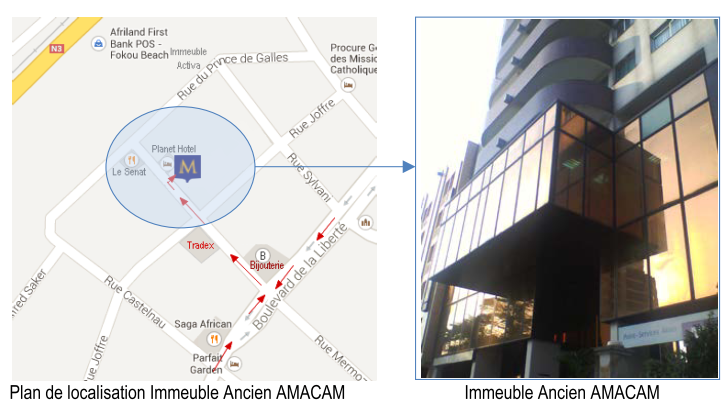
\includegraphics{localisation.png}

\subsection{Organisation générale de Mazars Cameroun}
Mazars Cameroun dispose de deux bureaux sur l’ensemble du territoire : 
\begin{itemize}
    \item Un bureau situé à Douala;
    \item Un second bureau situé à Yaoundé.
\end{itemize}
Notons que Mazars Cameroun est scnindé en deux principales unités:
\begin{itemize}
    \item Mazars Cameroun SA;
    \item Mazars TAX/LEGAL SA.
\end{itemize}
\begin{center}
    \begin{tabular}{c|c}
        \hline
         \textbf{Dénomination} & Mazars Cameroun SA  \\
         \textbf{Capital Social} & Vingt millions FCFA (20 000 000 FCFA) \\
         \textbf{Forme Juridique} & Société Anonyme (SA) \\
         \textbf{Boîte Postale} & 3791 Douala-Cameroun \\
         \textbf{Localisation} & Avenue Rue de Lapeyrere, Ancien Immeuble AMACAM, Douala \\
         \textbf{PDG} & M. Lucien Riquier \\
         \textbf{Logo} & 
\includegraphics{logo_M.png}
    \end{tabular}
\end{center}

\subsection{Secteur d'activité de Mazars Cameroun}
Mazars Cameroun est un cabinet d’expertise comptable qui fournit les lignes de service suivantes :
\begin{itemize}
    \item [-] Financial Audit
    \begin{itemize}
        \item[+] Audit légal
        \item[+] Audit contractuel
    \end{itemize}
    \item[-] Consulting
    \begin{itemize}
        \item[+] Gouvernance et maîtrise des risques
        \item[+] Stratégie et Opération
        \item[+] Développement durable
    \end{itemize}
    \item[-] Accounting and Outsourcing Services
    \begin{itemize}
        \item[+] Support fonction comptable et financière
        \item[+] Consolidation et \textit{Reporting}
        \item[+] Paie
        \item[+] Formalités fiscales
        \item[+] Sécrétariat juridique
    \end{itemize}
    \item[-] Financial Advisory Services
    \begin{itemize}
        \item[+] Litiges et fraudes
        \item[+] Financement de projet
        \item[+] \textit{Restructuring}
        \item[+] \textit{Transaction}
        \item[+] Modélisation et évaluation
    \end{itemize}
    \item[-] Tax Consulting
    \begin{itemize}
        \item[+] Fiscalité internationale-Douane
        \item[+] Fusion-Acquisition
        \item[+] Prix de transfert
    \end{itemize}
    \item[-]Legal Consulting
    \begin{itemize}
        \item[+] Droit des sociétés
        \item[+] Procédures collectives
        \item[+] Fusions et acquisitions
        \item[+] Banques et finances
        \item[+] Droit du travail
    \end{itemize}
\end{itemize}

\subsection{Présentation du département Consulting}
Notre stage s’est déroulé au sein du département consulting.  L’utilisation de plus en plus de l’outil informatique dans l’environnement de l’entreprise permet d’augmenter les chances d’atteindre leurs objectifs stratégiques. Toutefois, il faut associer à cela des dépenses substantielles dans le développement, l’implémentation et la maintenance de la technologie. 

Le département du Consulting a pour objectifs d’accompagner les clients à établir l’assurance que :
\begin{itemize}
    \item[-] \textbf{-	Les risques organisationnels clés sont correctement identifiés et évalués;}
    \item[-] \textbf{-	Les contrôles en place sont effectifs;}
    \item[-] \textbf{-	Les informations traitées sont conformes et sécurisées.}
\end{itemize}
Les Services offerts par ce département sont :
\begin{itemize}
    \item[-] \textbf{Audit}
    \begin{itemize}
        \item[+] Fonction informatique
        \item[+] Projets informatique
        \item[+] Exploitation
        \item[+] Applications opérationnelles
        \item[+] Sécurité informatique
    \end{itemize}
    \item[-] \textbf{Projects}
    \begin{itemize}
        \item[+] Diagnostic IT
        \item[+] Maturation des projets
        \item[+] Aide au choix de solutions IT
        \item[+] Mise en oeuvre
        \item[+] Conduite du changement
        \item[+] Accompagnement opérationnel
    \end{itemize}
    \item[-] \textbf{Sécurité de l'information}
    \begin{itemize}
        \item[+] Evaluation des vulnérabilités
        \item[+] Tests d'intrusion
        \item[+] Accompagnement ISO 270001
        \item[+] Revue Architecture de Sécurité
        \item[+] Analyse et Gestion de risques
        \item[+] Séminaire de formations
    \end{itemize}
\end{itemize}

\section{Etude de l'existant}
\subsection{Analyse Post-interviews}
Des interviews ont été réalisées au sein de chaque département de l'entreprise et les il est ressorti des ces interviews des éléments qui seront présentés dans la suite.
\subsubsection{Remarques}
Le département RH possède déjà un certain nombre de procédures rédigées. Cependant, ces procédures datent de 2013 et n’ont pas été mises à jour depuis cette date. Il convient donc de mettre à jour ces procédures afin de les aligner à la règlementation en vigueur. Les autres départements n’ont pas de procédures rédigées et validées.
\subsubsection{Actifs supports les plus sollicités au sein de l’entreprise}
\begin{itemize}
    \item[-] \textbf{Le serveur de messagerie:} qui permet d’échanger les mails au sein du cabinet mais aussi avec des entités externes;
    \item[-] \textbf{Le Serveur NAS :} : lieu de stockage de tous les documents numériques de l’entreprise : il s’agit en effet de la ressource la plus critique au sein de la structure et un niveau de protection adéquat doit être défini pour ce dernier ;
    \item[-] \textbf{Audisoft :} Il s’agit du logiciel utilisé dans le cadre des missions d’Audit. En communiquant avec son serveur GESTRAS il permet de mener à bien ces missions en stockant et en générant les fichiers nécessaires à l’accomplissement de la mission ;
    \item[-] \textbf{SAGE PAIE : }logiciel de gestion de la paie, il permet de gérer tous les paramètres liés à la paye des employés de Mazars mais aussi des clients ;
    \item[-] \textbf{SenatorFxLite : }logiciel de gestion des accès, gère les entrées et sorties au sein du cabinet ;
    \item[-] \textbf{PARRABELLUM : }logiciel de gestion des temps passés, permet de renseigner les temps passés sur une mission ou au sein du cabinet.
\end{itemize}
\subsubsection{Eléments redondants}
Nous avons remarqué que le processus d’archivage ne diffère pas vraiment d’un corps de métier à l’autre. En effet la seule différence remarquable se situe au niveau du temps de conservation après archivage ; mis à part ce détail, le processus reste le même.

\subsection{Etude comparative avec des solutions existantes}
La classification des données est essentielle pour les entreprises car elle permet de mieux protéger les informations détenues par l’entreprise. La classification des données permet aux utilisateurs d’attribuer une étiquette visuelle aux données qu’ils créent, de sorte que des décisions adéquates puissent être prises quant à leur manipulation (création, stockage, partage, suppression, etc.).

Les solutions de classification qui existent à l’heure actuelle consistent essentiellement en solutions logicielles. D’un autre côté, une autre approche consiste à adopter une démarche méthodologique afin d’aboutir à une politique de classification sur papier. Enfin une dernière approche consiste en une classification des données pilotée par l’utilisateur.[5]

\subsubsection{Utilisation d'un outil de classificaton automatisé}
La classification automatisée est basée sur un logiciel ou outil qui assiste l’utilisateur dans la classification réussie et précise de leurs fichiers de données. Cette classification peut être [6]:
\begin{itemize}
    \item[-] Entièrement automatisée;
    \item[-] Suggéré;
    \item[-] Prescite;
    \item[-] Approuvé par l'utilisateur.
\end{itemize}
Cette classification s’appuie en général sur des informations telles que l’emplacement de stockage des données, leur accessibilité, leur création et même leur contenu pour classer les données. Cette classification se fait généralement de la manière suivante :
\begin{itemize}
    \item[-] Ajout de métadonnées suivant le dossier dans lequel le document est stocké ;
    \item[-] Ajout de métadonnées suivant le lieu de stockage du document ;
    \item[-] Scan des documents afin d’identifier les sujets et thèmes desquels une classification sera suggérée ;
    \item[-] Ajout d’éléments visuels de marquage (en tête, pied de page, filigrane).
\end{itemize}

\textbf{Avantages d'une solution automatisée}
\begin{itemize}
    \item[-] Rapide retour sur Investissement car les résultats seront produits dans des délais assez courts ;
    \item[-] Réduction des erreurs humaines ;
    \item[-] Pas besoin d’une large communication ni de programmes de formation.
\end{itemize}

\textbf{Inconvénients d'une solution automatisée}
\begin{itemize}
    \item[-] Incompréhension du contexte de travail ce qui peut engendrer des sorties inexactes ;
    \item[-] Production de faux positifs qui peuvent entraver les processus métiers ;
    \item[-] Production de faux négatifs qui peuvent entraîner une perte de données.
\end{itemize}

\subsubsection{Classification des données par l'utilisateur}
Ici, les employés sont responsables de décider quelle étiquette est appropriée pour une information ; cet attachement se fait à travers un logiciel au moment de la création, envoi, modification ou enregistrement du fichier.
\textbf{Avantages}
\begin{itemize}
    \item[-] L’utilisateur est plus impliqué dans le contexte ce qui lui permet de définir correctement l’étiquette à appliquer à une donnée ;
    \item[-] Il s’agit d’une couche de sécurité supplémentaire utilisée souvent pour compléter la classification automatisée.
\end{itemize}
L'inconvénient de cette approche est qu'elle prend du temps pour être mise en place. Les employés doivent être formés afin de connaître exactement quelle étiquette associer à une information.

\subsubsection{Politique de classification sur papier}
Il s’agit ici d’élaborer une politique de classification que chaque employé manipulant des informations devra utiliser afin d’étiqueter celles-ci. Dans cette approche l’on doit s’assurer que les employés s’alignent à cette politique et à la politique globale de sécurité de l’entreprise. Une politique bien définie permet aux employés de prendre rapidement des décisions intuitives quant à l’étiquette à fournir à une donnée. 

L’inconvénient avec cette approche qui n’a aucun soutien technologique est qu’il faut mettre en place des contrôles pour s’assurer que tout le monde est au courant de la politique et la met en place. 

Le tableau de comparaison ressort les différences et corrélations entre les solutions de classification existantes suivants un ensemble de critères bien définis.
\begin{center}
    \begin{tabular}{c|c|c|c}
        \hline
         \textbf{Critère de comparaison} & \textbf{Classification automatisée} & \textbf{Classification dirigée par l'utilisateur} & \textbf{Classification sur papier}  \\
        \hline
         Rapidité des résultats fournis & Grande & Moyenne & Faible \\
         \hline
         Fiabilité des résultats & Moyenne & Grande & Moyenne \\
         \hline
         Réduction des erreurs humaines & Grande & Grande & Faible \\
         \hline
         Compréhension du contexte de travail & Faible & Moyenne & Grande \\
         \hline
         Taux de faux positifs & Grand & Faible & Faible \\
         \hline
         Taux de faux négatifs & Grand & Faible & Faible \\
         \hline
         
    \end{tabular}
\end{center}

\part{Conception de la solution et mise en oeuvre}

%!TEX root =  tfg.tex
\chapter{Conception de la solution et mise en oeuvre}

\begin{quotation}[Novelist]{Ernest Hemingway (1899--1961)}
The good parts of a book may be only something a writer is lucky enough to overhear or it may be the wreck of his whole damn life -- and one is as good as the other.
\end{quotation}

\begin{abstract}
Resumen de lo que va a ocurrir en el capítulo. ¿Cuál es el objetivo que tenemos con este capítulo?
\end{abstract}

\section{Réalisation de la cartographie des données}
\subsection{Problématique}
Le problème ici est de pouvoir tracer le parcours d’une donnée depuis son entrée dans l’entreprise jusqu’à sa sortie ou sa destruction. Comment est créée l’information ? Où est-elle stockée ? Combien de temps est-elle stockée ? Quel est son procédé de destruction ? Qui a accès à cette information ? Comment cette information est-elle gardée en sécurité ?

\subsection{Cartographie}
Pour se faire l’on doit recenser un certain nombre d’éléments lors de la cartographie des processus :
\begin{itemize}
    \item[-] \textbf{Le nom de l’information : }identifiant unique de l’information au sein de l’entreprise ;
    \item[-] \textbf{Le propriétaire de l’information : }responsable de la gestion de l’information ;
    \item[-] \textbf{Le format de l’information : }format physique ou numérique principalement ;
    \item[-] \textbf{Les responsabilités liées à l’information : }Propriété, entités qui y accèdent et droits d’accès ;
    \item[-] \textbf{L’impact que l’information peut avoir sur l’entreprise : }conformité, opérationnel, réputation, financier ;
    \item[-] \textbf{Ses besoins de sécurité : }en termes de confidentialité, d’intégrité et de disponibilité ;
    \item[-] \textbf{Canaux de diffusion : }SIs sollicités, systèmes et réseaux utilisés pour le transfert de l’information ;
    \item[-] \textbf{Les règles de marquage applicable :}lois et règles applicables sur l’information ;
    \item[-] \textbf{Le cycle de vie de la donnée : }temps de conservation jusqu’à étape du processus
    \item[-] \textbf{Le support de stockage : }Cloud, Bases de données, serveurs…
    \item[-] \textbf{La conservation : }temps de conservation total de l’information ;
    \item[-] \textbf{Le procédé de destruction de l’information ;}
    \item[-] \textbf{Les mesures de sécurité appliquées dans l’entreprise.}
\end{itemize}
Un extrait de cette cartographie est fournie dans un document annexe nommé « Cartographie des traitements ».

Il est important de faire ressortir les échelles de classification suivant les 3 principes de la sécurité : confidentialité, intégrité, disponibilité. Le tableau ci-dessous fournit les échelles de classification que nous avons retenue :

\begin{center}
    \begin{tabular}{|c|c|c|c}
        \hline
        \multicolumn{4}{|c|}{Echelle de confidentialité} \\
         Confidentialité & Description de l'expression du besoin & Niveau d'impact redouté & Exemple  \\
         Confidentiel & Information ayant un impact significatif sur l’entreprise si elle était amenée à être divulguée en dehors de personnes identifiées & 4 & Préparation d’une nouvelle offre de service \\
         A usage restreint & Information dont l’accès est restreint au personnel (interne) impliqué & 3 & Dossier de mission \\
         A usage interne & Information dont la divulgation en dehors de l’entreprise peut nuire à celle ci & 2 & Organigramme  l’entreprise \\
         Public & Information qui peut être rendue publique sans impact pour l’entreprise ou l’entité associée & 1 & Adresse du cabinet \\
         \hline
        \multicolumn{4}{|c|}{Echelle d'Intégrité} \\
        Intégrité & Description de l'expression du besoin & Niveau d'impact redouté & Exemple \\
        Elevé & Information dont l’altération provoquerait un impact élevé sur l’entreprise & 3 & Données financières de l'entreprise\\
        Moyen & Information dont l’altération aura un impact important sur l’entreprise & 2 & Contenu du site internet de Mazars Cameroun \\
        Faible & Toute altération de l’information aura un impact faible sur l’entreprise & 1 & Livret de présentation Mazars Cameroun \\
        \hline
        \multicolumn{4}{|c|}{Echelle de disponibilité}\\
        Disponibilité & Description de l'expression du besoin & Niveau d'impact redouté & Exemple \\
        Elevé & Indisponibilité non tolérée. Toute indisponibilité aura un impact élevé sur l’entreprise & 3 & Serveur de messagerie \\
        Moyen & Toute indisponibilité aura un impact important sur l’entreprise & 2 & GESTRAS \\
        Faible & L’indisponibilité a un impact faible pour l’entreprise & 1 & Site Web \\
        \hline 
    \end{tabular}
\end{center}
\section{Modélisation des processus métier}
Le tableau ci-dessous présente un récapitulatif des processus métiers que l’on a pu recenser suivant le corps de métier au sein de la structure.
\begin{center}
    \begin{tabular}{|c|c|}
        \hline
         Corps de métier & Nom du processus  \\
         \multirow{8}{4em}{Ressources Humaines} & Recrutement \\
         &Mise en Service \\
         & Envoi en formation \\
         & Traitement de la paie \\
         & Gestion des évaluations \\
         & Départ en congés \\
         & Renvoi/Démission \\
         & Archivage \\
         \hline
         \multirow{4}{2em}{Tax/Legal} & Ouverture d'une mission \\
         & Organisation des documents collectés pour une mission \\
         & Clôture d’une mission \\
         & Archivage \\
         \hline
         \multirow{6}{2em}{Audit} & Création d'une mission \\
         & Traitement du dossier d’audit \\
         & Gestion du dossier de mission \\
         & Gestion du dossier permanent \\
         & Gestion de la fin d’une mission \\
         & Archivage \\
         \hline
         \multirow{3}{2em}{Equipe IT} & Stockage \\
         & Sauvegarde \\
         & Archivage \\
         \hline
         \multirow{2}{2em}{Administration et Finances}
         & Traitement des informations bancaires et financières \\
         \hline
         Business Development & Traitement des données utilisées pour les appels d’offres, proposition de service \\
    \end{tabular}
\end{center}
La description de chaque processus est fournie dans l’annexe « Cartographie des traitements ».
\textit{Département RH}
Le département RH possède déjà ces propres processus, l'on a donc proposé des améliorations aux processus existants.

\textit{Département Audit}
\textit{Département Tax/Legal}
\textit{Administration et Finances}
\section{Rédaction des procédures}
A la suite de la classification effectuée, sur la base des besoins en sécurité des biens essentiels et sur les mesures de sécurité à mettre en place, nous avons rédigé des procédures renseignées dans le « Manuel de procédures » de l’entreprise.

\section{Mise en oeuvre des procédures}
\textbf{Plan de déploiement}
\begin{tabular}{c|c}
    Responsables des mesures de sécurité identifiées & Le délégué à la protection des données(DPO)  \\
     Echéances de déploiement & Aucune échéance ne peut être fournie car toutes les politiques et procédures n’ont pas encore été mises en place \\
     Ressources nécessaires & - \\
     Propriétaires de l'information & Délégué à la protection des données \\
     Responsable du suivi et du maintien de la classification & Délégué à la protection des données \\
     Parties prenantes impliquées dans la revue de la classification & \begin{itemize}
         \item[-] Délégué à la protection des données (DPO)
         \item[-] Tout membre du personnel ayant été sensibilisé sur la classification des données
     \end{itemize}\\
\end{tabular}
%saut de page
%!TEX root =  tfg.tex
\chapter{Conclusiones}

\begin{quotation}[Novelist]{Ernest Hemingway (1899--1961)}
The good parts of a book may be only something a writer is lucky enough to overhear or it may be the wreck of his whole damn life -- and one is as good as the other.
\end{quotation}

\begin{abstract}
Resumen de lo que va a ocurrir en el capítulo. ¿Cuál es el objetivo que tenemos con este capítulo?
\end{abstract}

\section{Rappel du problème}

Le problème qui nous a été posé avait deux volets ; premièrement mettre en place une solution de classification des données manipulées par Mazars Cameroun. Suite à cette classification, rédiger des politiques et procédures qui permettront d’assurer la conformité de Mazars Cameroun au RGPD ainsi qu’aux autres lois sur la protection des données.

\subsection{Bilan}
Au terme de notre stage, nous avons proposé une classification des différentes informations que l’on a pu recenser, ce suivant l’échelle de classification fournie plus haut et suivant l’impact que pourrait avoir cette information si son besoin en sécurité venait à être modifié. Cette classification a été établie dans un document appelé « Cartographie des traitements » qui associe à chaque information un marquage approprié (confidentiel, public, etc.). En plus de ce document de classification nous avons fourni le « registre de traitements ». Notons que l’article 30 du GDPR impose la tenue d’un registre de traitement qui contient un certain nombre d’informations sur les traitements impliquant les données personnelles. 

En plus, nous avons renseigné dans un « Manuel de procédures » un certain nombre de tâches à exécuter afin de pouvoir réaliser les processus métiers au sein de l’entreprise et ce en respect de la règlementation en vigueur. 

\subsection{Acquis personnels et difficultés rencontrées}
Ce stage nous a permis:
\begin{itemize}
    \item[-] D'améliorer notre sens de la communication à travers les interviews menées;
    \item[-] De découvrir le RGPD et d’augmenter notre niveau de connaissances en matière de protection des données (notamment dans la mise en place de mesures de sécurité appropriées) ;
    \item[-] D’acquérir des connaissances sur le fonctionnement global d’un cabinet d’Audit, ainsi que les responsabilités liées au travail en cabinet.
\end{itemize}
Difficultés rencontrées:
\begin{itemize}
    \item[-] La sensibilisation du personnel n’a pas été effectuée : ainsi, pendant les interviews les éléments collectés n’étaient pas toujours pertinents car les intervenants n’avaient pas été préparés à notre venue;
    \item[-] Les interlocuteurs n’avaient n’étaient pas toujours qualifiés ou bien informés pour répondre à nos questions, ceci due à l’indisponibilité des chefs de départements;
    \item[-] -	Mis à part le département des Ressources Humaines, aucun autre département n’avaient des procédures rédigées et validées ; cela est la cause de l’importance du temps que nous avons mis à recenser les éléments qu’il fallait pour les procédures.
\end{itemize}

\subsection{Perspectives}
Dans un souci d’amélioration de ce qui a été fait jusqu’ici, il conviendrait de :
\begin{itemize}
    \item[-]Renseigner dans le manuel de procédures toutes les procédures recensées au sein de l’entreprise car ce n’est qu’une partie des procédures qui a été rédigée ;
    \item[-]Migrer vers une solution automatique de classification des documents, celle-ci aura pour principal objectif de marquer les documents (Word, Powerpoint, etc.) à chaque niveau de leur cycle de vie ;
    \item[-] Pouvoir identifier le lieu de stockage de chaque donnée au sein de l’entreprise, et tenir en compte le fait qu’elle ait pu être dupliquée ;
    \item[-] Mettre en place des politiques de suppression des données conformément au RGPD ;
    \item[-] Automatiser un certain nombre de processus afin de faciliter la traçabilité des données manipulées et afin de se rassurer que les procédures sont respectées.
\end{itemize}





%Saut de page ici
\appendix

%!TEX root =  tfg.tex
\chapter{Software Product Lines}

\begin{quotation}[Novelist]{Ernest Hemingway (1899--1961)}
The good parts of a book may be only something a writer is lucky enough to overhear or it may be the wreck of his whole damn life -- and one is as good as the other.
\end{quotation}

\begin{abstract}
This is an example of an abstract. Multiple lines are supported. Several paragraphs. It jumps to the next page. Blau blau blau. I am  introducing more text to reach the third line 
\end{abstract}



\section{Software Product Lines}

\begin{itemize}
\item Objective of a \Gls{pl} (mass production and customisation) \cite{benavides05-CAISE}
\item The focus in software derives in \Glspl{spl}.
\item Variability management: variability models
\item When and how are used VMs: FMs are described in FODA report as a key element in SPL since they represent the variability and commonality of the different products in a SPL.
\end{itemize}

\section{Feature Models}
\todo[inline]{To Abductive Section in 2.1}

As the number of products to be built by a SPL may be large and the constraints among features may be complex, representing such an information in a manageable and compact manner is a must. \fms represent the set of products a SPL may build in terms of product features. Some features are optional while others are mandatory. To indicate the relationships among features, they are hierarchically linked, forming a tree whose root is a feature representing the whole functionality of a product. The root feature is refined in child features, which increase the level of detail and reduce the scope of features. Recursively following this refinement process, a tree-like structure is obtained where three basic kinds of hierarchical relationships are used:
\begin{itemize}
\item Mandatory: a mandatory relationship affects a parent and child feature. It forces the child feature to appear in a product whenever its parent feature does. 
\item Optional: a child feature connected to a parent feature by means of an optional relationship may be optionally selected whenever its parent feature is.
\item Set-relationships: three or more features are part of a set-relationship: a parent feature and a set of two or more child features. A set-relationship contains a cardinality that constraints the number of child features to be selected in a product whenever its parent feature is selected. If the cardinality is $[1..1]$ it is commonly remarked as an \emph{alternative relationship} where only one child feature may be selected at the same time. If the cardinality is $[1..N]$ (where $N$ is the number of child features), it is also known as an \emph{or-relationship} as any combination of child features is allowed while at least one is selected.
\end{itemize}

Although \fms can represent most of the most frequent constraints, the hierarchical nature of these models might hinder the representation of some constraints. Under this circumstance, \emph{cross-tree constraints} can be added. The most common kinds of cross-tree constraints are:
\begin{itemize}
\item Dependency: a feature depends on another feature if the second one must be part of a product whenever first one is selected.
\item Exclusion: two features exclude themselves if both of them cannot be part of a product at the same time.
\end{itemize}

\begin{figure*}[htb]
	\centering
		\missingfigure{A feature model example}
		%\includegraphics[width=1.00\textwidth]{figures/reasoning.pdf}
		\caption{An example of a Home Integration System\label{fig:FMexample}}
\end{figure*}

The example in Figure \ref{fig:FMexample} describes a \emph{Home Integration System} (HIS) \spl in terms of its features and the relationships among them. Leaning on this example we define some useful terms:

\begin{description}
\item[Partial configuration] : a partial configuration is a composed by three sets of selected ($S$), removed($R$) and undecided($U$) features.  A feature can only be in one of these sets and every feature in the \fm ($fm$) must be in one of them, i.e. $S \cup R \cup U = fm$ and $S \cap R \cap U = \emptyset$. A partial configuration represents an intermediate state during the process of a customer selecting the feature for a custom product. For example, $S_P=\{...\}$, $R_P=\{...\}$ and $U_P=\{...\}$ define a partial configuration for the sample \fm where some features are still to be decided if they are to be selecter or removed in a configuration.
\end{description}

\begin{description}
\item[(Full) configuration] : a full configuration or simply a configuration is a partial configuration such that the set of undecided features in empty. For example, $S_F=\{...\}$ and $R_F=\{...\}$ describe a full configuration for the example \fm.
\end{description}

\begin{description}
\item[Product] : a product is a representation for a full configuration such that only the selected features are remarked. For instance, $P=\{\}$ is a product for the above full configuration. A product such as \texttt{A,B} is a valid since all the constraints within the \fm are satisfied. However, A,B and C is not a valid product since D is required.
\end{description}

\begin{description}
\item[Validation]
A partial configuration is \emph{valid} if all the relationships and constraints are satisfied given the sets of selected, removed and undecided features. So the definition applies for valid full configurations and valid products. As a conclusion we can affirm that a FM represents all the valid products in a SPL.
\end{description}

\objective{Briefly expose attributes as an important asset in feature models.}
It is frequent that features are not enough to represent information that is relevant to represent a \spl variability. In this case, \fms are extended with feature attributes such as cost, versions, RAM consumption, etc. in the so-called \Glspl{efm} \cite{benavides05-CAISE}. Besides relationships, an \Gls{efm} contains constraints that affect attributes which reduce even more the set of products a \fm describes. Above definitions remain when attributes are introduced into \fms. 

\section{Automated Analysis of Feature Models}

\subsection{Scope}
\todo[inline]{To Abductive Intro}

FMs are used all along the SPL development as key models and many of the development decisions are taken relying on the information contained within them. Most of the times, relationships are complex and hinder the manual extraction of information. Manually obtaining information such as 'which is the product that costs the less?', 'does the feature model contain errors?' or 'why there exist no product containing certain features?' can be an unfeasible task. The complexity and compactness of FMs justify the need of an automated support of these operations. So the \textit{Automated Analysis of Feature Models} (AAFM) arises as a topic of interest to deal with this problem in the SPL community.

\sidebox{Use me to explain in a larger text than 'sidetext' anything that is important to a reader not familiar with the dissertation context for example.}

The AAFM can be seen as a black-box process that receives a FM and an operation as inputs and obtains information (its kind depends on the analysis operation) as an output (Fig. \ref{fig:oldBlackBox}). There are many operations that extract information from a FM such as 'counting products' operation whose result is a natural number indicating the number of customised products that can be built; or 'list of products' operation that obtains each of those products. This vision of AAFM as a black-box is valid for a subset of analysis operations that we call \emph{information extraction operations} (IEO) that can be seen as processes to extract information from FMs. In other words, an IEO makes explicit an implicit information within a FM. 

\begin{figure}[htb]
	\centering
	\subfigure[The AAFM seen as a black-box process]{
		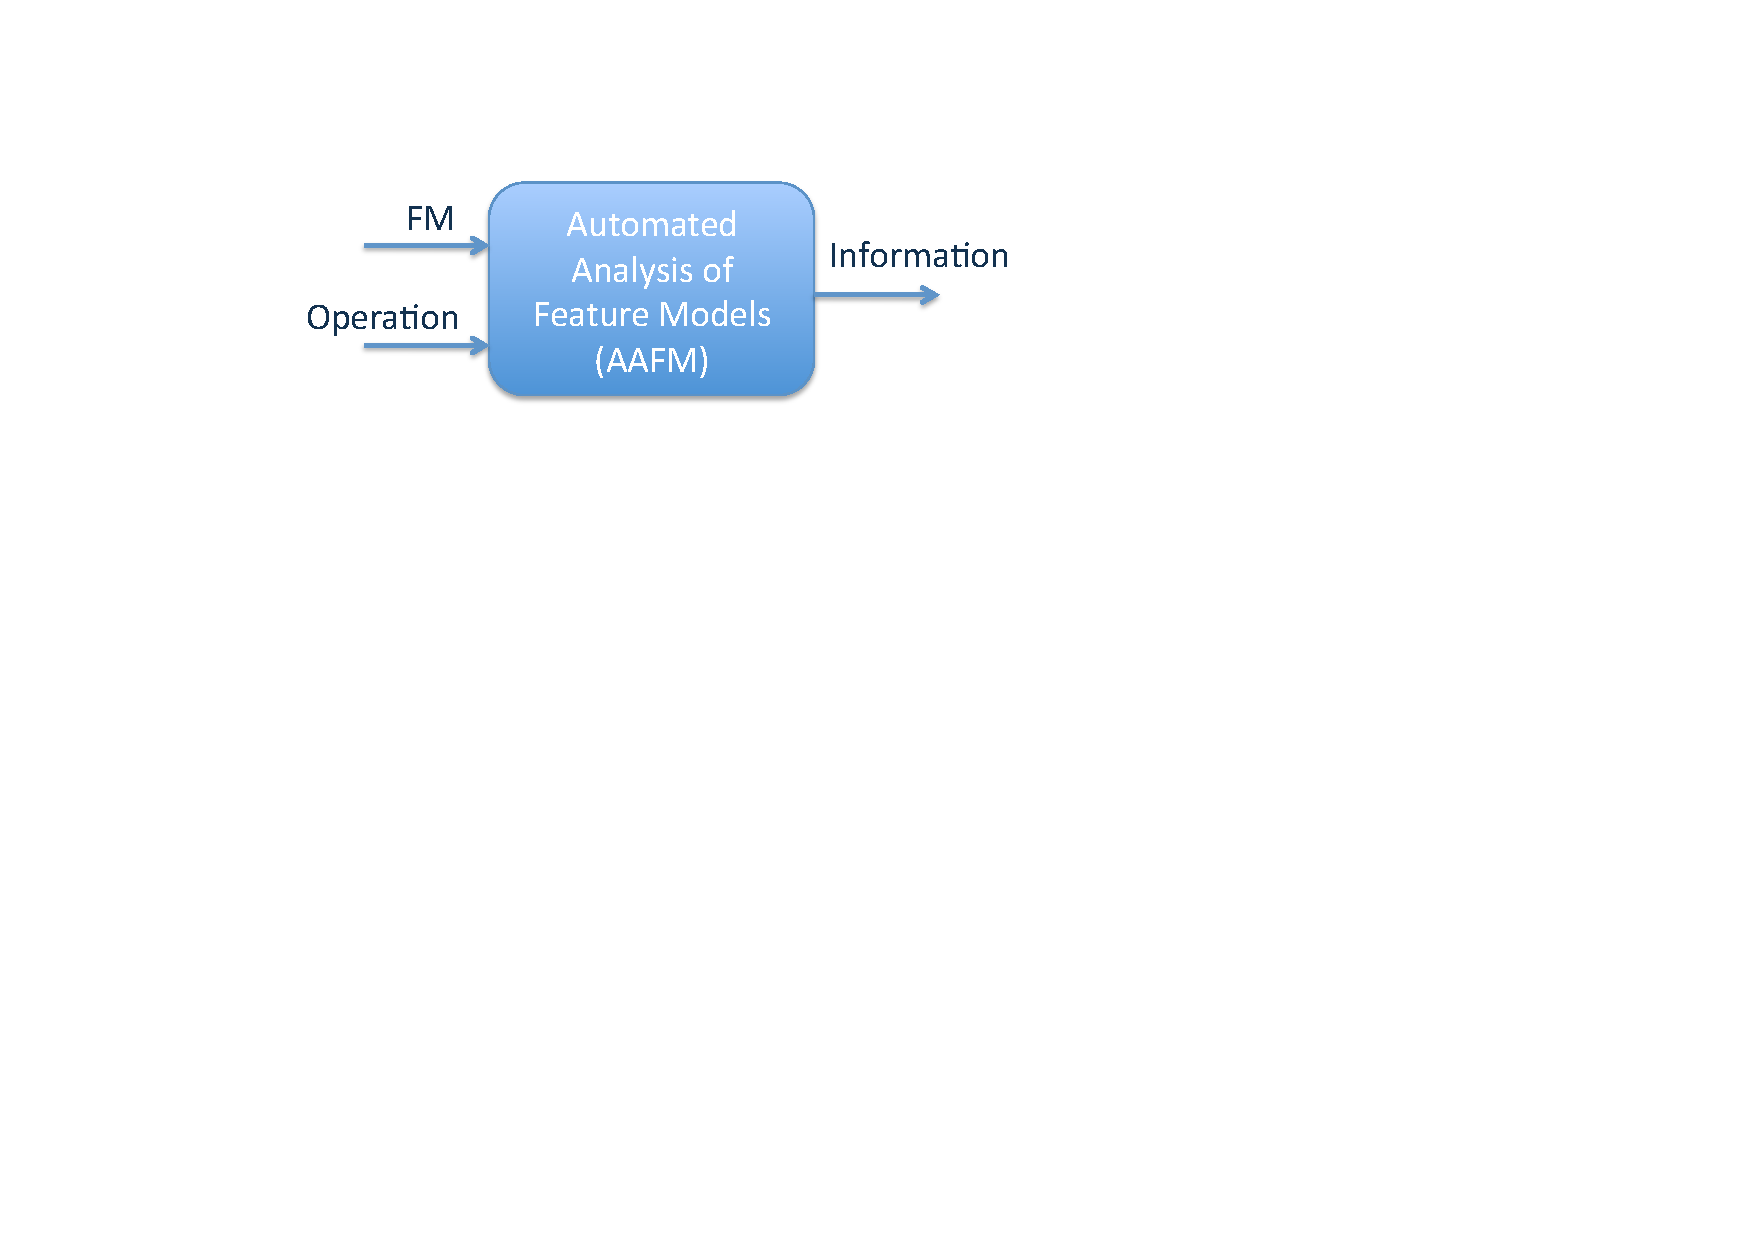
\includegraphics[width=0.30\textwidth]{figures/introduction/oldAAFM.pdf}
		\label{fig:oldBlackBox}
	}
		\subfigure[Extending the AAFM process with explanations]{
		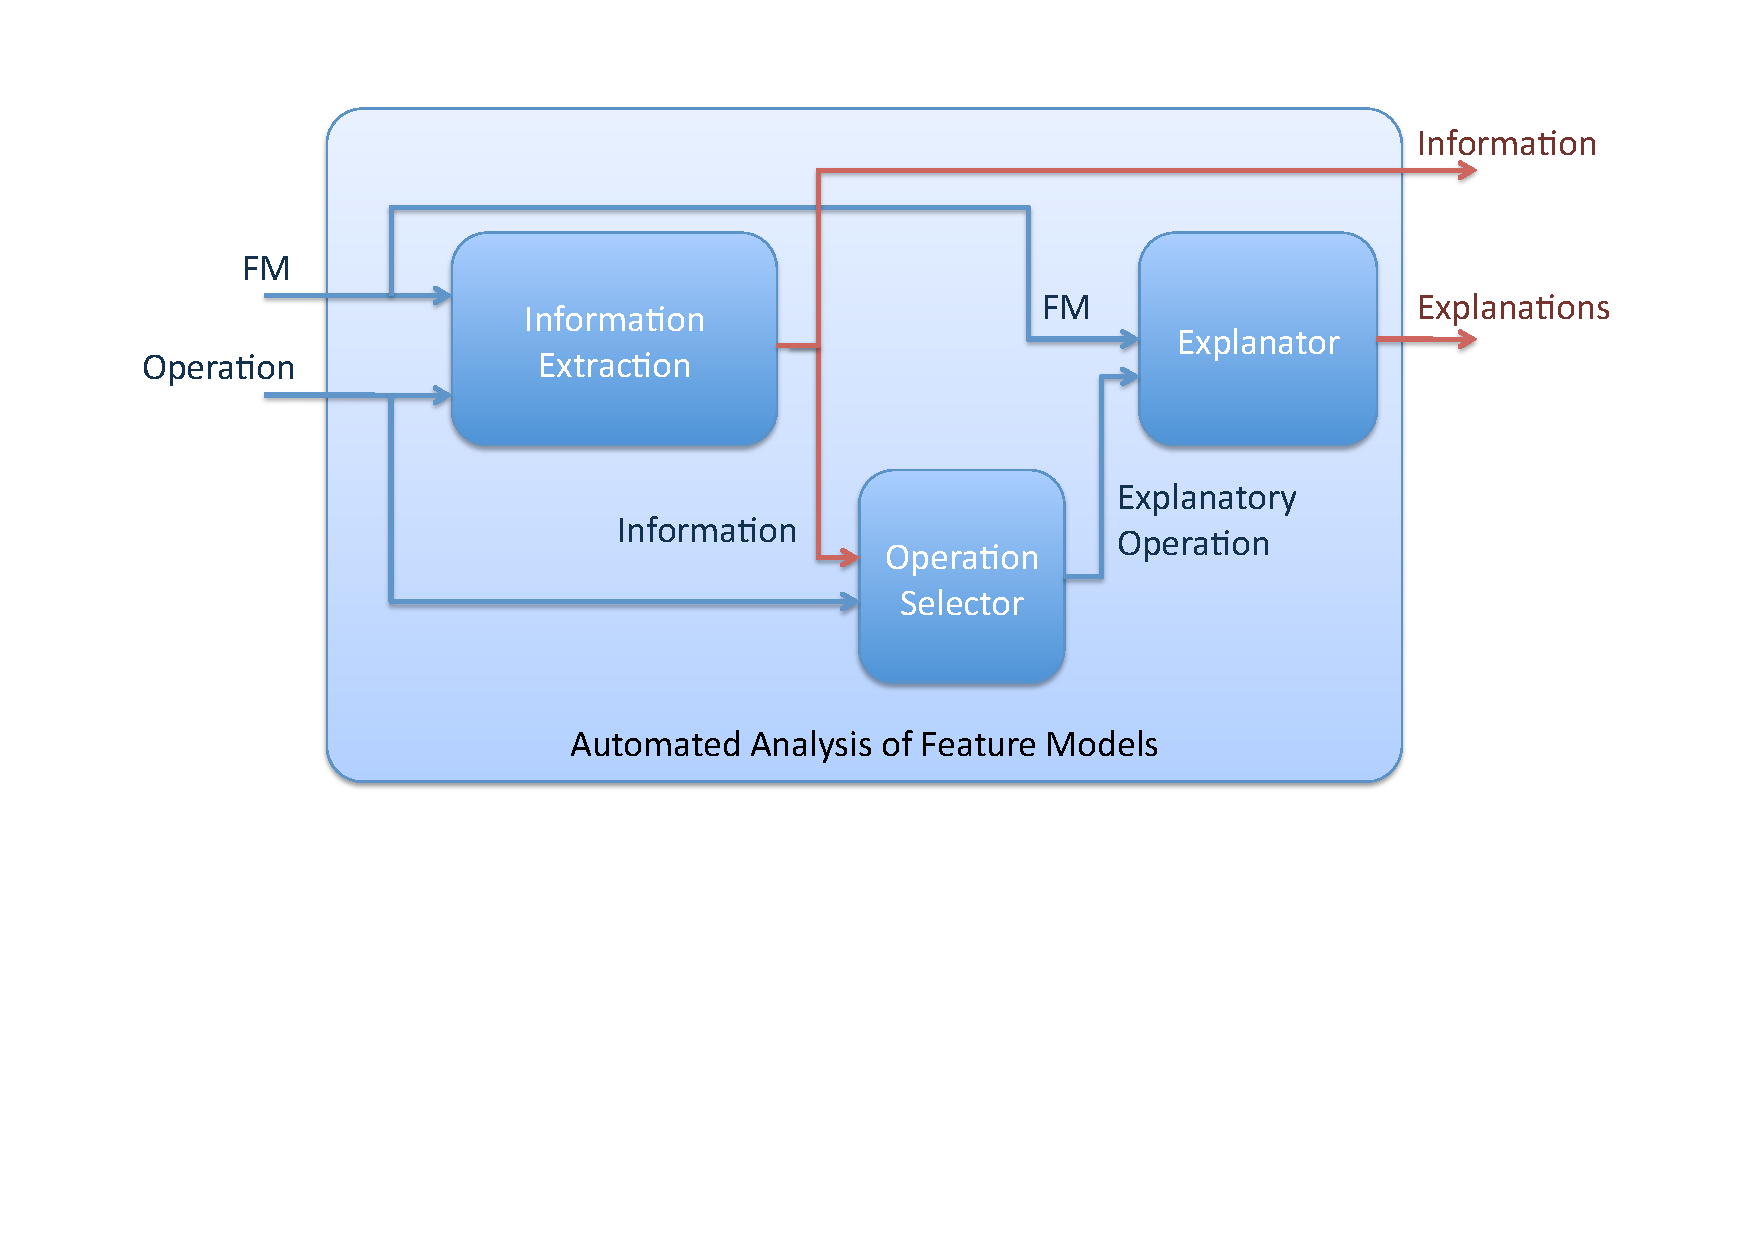
\includegraphics[width=0.65\textwidth]{figures/introduction/newAAFM.pdf}
		\label{fig:newBlackBox}
	}
		%\missingfigure{Several architectures and a structural model for each of them (Slide 3)}
		
	\caption{A different view on AAFM distinguishing between information extraction and explanatory operations}
	\label{fig:AAFM}
\end{figure}

However, there is a subset of analysis operations known as \emph{explanatory operations} (EO) whose objective is explaining the result obtained from a IEO. Sometimes, the result is not the expected one and the analyser needs to know which are the relationships that have caused it. For example, let us suppose that the IEO 'which are the products described in a FM that cost less than \$1000?' obtains no products as a result. If we were expecting to obtain at least one product, it is important to determine the relationships in the FM that are responsible of that behaviour, so an EO 'why there is no product costing less than \$1000?' will shed light on the relationships that avoid obtaining any product. Obtaining no result is not the only case that claims for explanations. If we obtained only one product as a result and we were expecting to obtain at least 10 products, although an answer is obtained the result is unexpected and the discrepancy reasons have to be found. Moreover, explanatory operations are also useful even when an expected result is obtained, to reinforce the certainty that the result is correct. So it can be concluded that EOs complement the information an FM analyser obtains from IEOs.

The complexity of feature modelling relies on correctly setting the relationships that describe the set of products to be built in a SPL. Relationships are the only elements responsible of the results obtained in FM analysis. So an \emph{explanation} is a set of relationships that may have caused that result. While IEO provides for an unique response that is known for certain, an EO provides for a set of probable explanations to a result obtained from a IEO, being only one of them a valid explanation. It would be the analyser the one in charge of discriminating the correct explanation, maybe performing new analysis operations.

\sidetext{This is a side text. Use to remark important information}

Therefore, two kinds of operations are distinguished in AAFM: information extraction and explanatory operations. Explanatory operations have no sense without a paired information extraction operation and its result. To ensure that explanatory operations are always paired to an information extraction operation, we define a new black-box process of AAFM that incorporates explanations as an additional output (see Figure \ref{fig:newBlackBox})

\begin{enumerate}
\item Information extraction: the original process, which remains the same.
\item Operation selector: depending on the information extraction operation the analyser asks for and the information obtained as a result, this process provides the explanatory operation to be performed. In other words, it pairs an explanatory operation to an information extraction operation.
\item Explanatory analysis: provides a set of explanations from the FM and the explanatory operation.
\end{enumerate} 

The overall process can be encapsulated into a holistic black-box process which receives the FM and the information extraction operation as inputs and provides a result and explanations as outputs. It can be seen as we just add explanations as an output to the analysis process. 

To realise this view on the AAFM, we need to give details on the insides of these black-boxes. Since the information extraction process is already rigourously defined in Benavides' PhD dissertation, the purpose of this paper is defining the remaining two sub-processes. We formalise the explanatory analysis process by means of default logic and provide the criteria to implement the operation selector process.

Most Common Techniques to perform AAFM Operations.


\section{Dynamic Software Product Lines (DSPL)}
What is a \dspl. Different points of view. What is important is the automation of reconfiguration properties relying on \spl techniques.

We focus in the application of explanations in \dspls as an application of our results. Specifically we have worked in MAS and smart homes providing a solution for automating product reconfiguration.

\section{Hypothesis and Objectives}

\objective{Justifying that explanations are a particular set of operations in AAFM that are not solvable by means of the techniques that are used up-to-date}
\objective{Set an impacting phrase that summarises the hypothesis}
\importantframe{Hypothesis}{Explanations cannot be solved by AI techniques used to solve AAFM. There should exist other AI techniques to solve explanations. }

\importantframe{Objective of the dissertation}{Defining a framework to provide solutions for explanatory analysis in FMs.}

This dissertation summarises our contribution to solve some of the objectives we set in our PhD project. 

\begin{itemize}
\item Defining a catalog of analysis operations where explanations are applied.
\item Rigorously defining these operations in terms of logics.
\item Proposing solutions to these operations.
\item Validating our results by means of tools and projects where they are applied. 
\end{itemize}

Next chapter focuses on refining how we have contributed to deal with the above objectives.

A piece of code...

\begin{lstlisting}[style=javacode]
public Map<Cardinality,CardinalValue> detectWrongCardinals() {
	// any other implementation of Map can be used instead.
	Map<Cardinality,CardinalValue> result = 
		new TreeMap<Cardinality,CardinalValue>();
	for( r : relationships) {
		if (r instanceof Set) {
			Set set = (Set)r;
			Cardinality card = set.getCardinality();
			Domain dom = card.getDomain();
			for (value: dom.getValues())
				if (isWrongCardinal(card,value))
					result.put(card,value);
		}
	}
	return result;
}
\end{lstlisting}

A coolTable. Use inside a table.
\begin{table*}[h!]
	\centering
	\begin{coolTable}{lcc}{3} % 3 is the only addition to standard tabular environment
	% lcc is the alignment for each columns. 3 is the total number of columns of the table.
{A Catalog of FM Explanatory Operations (2009 version)}
			\textbf{Information Extraction Operation}&\multicolumn{2}{c}{\textbf{FM Explanatory Operations}}\\
			\midrule
			% Always use midrules instead of \hline. It adds an extra vertical space that helps to improve the clarity
			&\textit{Why? operation}&\textit{Why not? operation}\\
			\cmidrule(r){2-3} % use cmidrule instead of \cline.
			Valid FM&-&invalid FM \\
			Valid Configuration&valid partial conf.&invalid partial conf.\\		
			Valid Product&valid product&invalid product\\
			Products Listing&vaild Product/Config&invalid FM/Product/Config\\
			Products Counting&vaild Product/Config&invalid FM/Product/Config\\
			Optimisation&vaild Product/Config&invalid FM/Product/Config\\
			Core feature&core feature&core feature\\
			Variant feature&variant feature&variant feature\\
			Dead feature detection&-&dead feature\\
			False-optional feature detection&-&false-optional feature\\
			Wrong-cardinality detection&-&wrong cardinal\\
			%\multirow{2}{*}{\textbf{Information Extraction Operation}}
			\textbf{Information Extraction Operation}&\multicolumn{2}{c}{\textbf{Configuration Explanatory Operations}}\\
			\midrule
			&\textit{Why? operation}&\textit{Why not? operation}\\
			\cmidrule(r){2-3}
			Valid Configuration&valid partial conf.&invalid partial conf.\\	
		\end{coolTable}
	\caption{Most frequently used explanatory operations and their corresponding information extraction operations}
	\label{tab:listDeductiveAbductive}
\end{table*}

Use \textbackslash TableSubtitle\{n,title\} to add a subtitle as the header. n is the number of columns and title is the text to place. \citep{benavides05-CAISE}


\glossarystyle{long}
\printglossaries
\newpage

\bibliographystyle{abbrvnat}
\addcontentsline{toc}{chapter}{Referencias bibliográficas}
\bibliography{referencias}

\end{document} 